% move all configuration stuff into includes file so we can focus on the content
\documentclass[aspectratio=169,hyperref={pdfpagelabels=false,colorlinks=true,linkcolor=white,urlcolor=blue},t]{beamer}

%%%%%%%%%%%%%%%%%%%%%%%%%%%%%%%%%%%%%%%%%%%%%%%%%%%%%%%%%%%%%%%%%%%%%%%%%%%%%%%%%%
%%%%%%%%%%%%%%%%%%%%%%%%%%%%%%%%%%%%%%%%%%%%%%%%%%%%%%%%%%%%%%%%%%%%%%%%%%%%%%%%%%
% packages
\usepackage{pict2e}
\usepackage{epic}
\usepackage{amsmath,amsfonts,amssymb}
\usepackage{units}
\usepackage{fancybox}
\usepackage[absolute,overlay]{textpos} 
\usepackage{media9} % avi2flv: "C:\Program Files\ffmpeg\bin\ffmpeg.exe" -i TuneFreqFilterbank.avi -b 600k -s 441x324 -r 15 -acodec copy TuneFreqFilterbank.flv
\usepackage{animate}
\usepackage{gensymb}
\usepackage{multirow}
\usepackage{silence}
\usepackage[backend=bibtex,style=ieee]{biblatex}
\AtEveryCitekey{\iffootnote{\tiny}{}}
\addbibresource{references}

%%%%%%%%%%%%%%%%%%%%%%%%%%%%%%%%%%%%%%%%%%%%%%%%%%%%%%%%%%%%%%%%%%%%%%%%%%%%%%%%%%
%%%%%%%%%%%%%%%%%%%%%%%%%%%%%%%%%%%%%%%%%%%%%%%%%%%%%%%%%%%%%%%%%%%%%%%%%%%%%%%%%%
% relative paths
\graphicspath{{graph/}}


%%%%%%%%%%%%%%%%%%%%%%%%%%%%%%%%%%%%%%%%%%%%%%%%%%%%%%%%%%%%%%%%%%%%%%%%%%%%%%%%%%
%%%%%%%%%%%%%%%%%%%%%%%%%%%%%%%%%%%%%%%%%%%%%%%%%%%%%%%%%%%%%%%%%%%%%%%%%%%%%%%%%%
% units
\setlength{\unitlength}{1mm}

%%%%%%%%%%%%%%%%%%%%%%%%%%%%%%%%%%%%%%%%%%%%%%%%%%%%%%%%%%%%%%%%%%%%%%%%%%%%%%%%%%
%%%%%%%%%%%%%%%%%%%%%%%%%%%%%%%%%%%%%%%%%%%%%%%%%%%%%%%%%%%%%%%%%%%%%%%%%%%%%%%%%%
% theme & layout
\usetheme{Frankfurt}
\beamertemplatenavigationsymbolsempty
%\setbeamertemplate{frametitle}[smoothbars theme]
\setbeamertemplate{frametitle}
{
    \begin{beamercolorbox}[ht=1.8em,wd=\paperwidth]{frametitle}
        \vspace{-.1em}%
        \hspace{.2em}{\strut\insertframetitle\strut}
        
        \hspace{.2em}\small\strut\insertframesubtitle\strut
        %\hfill
        %
\includegraphics[height=.8cm,keepaspectratio]{CenterMusicTechnology-solid-2lines-white-CoAtag}
        
    \end{beamercolorbox}
    \begin{textblock*}{100mm}(11.6cm,.7cm)
        \includegraphics[height=.8cm,keepaspectratio]{logo_GTCMT_black}
    \end{textblock*}
}

% set this to ensure bulletpoints without subsections
\usepackage{remreset}
\makeatletter
\@removefromreset{subsection}{section}
\makeatother
\setcounter{subsection}{1}

%---------------------------------------------------------------------------------
% appearance
\setbeamercolor{structure}{fg=gtgold}
\setbeamercovered{transparent} %invisible
\setbeamercolor{bibliography entry author}{fg=black}
\setbeamercolor*{bibliography entry title}{fg=black}
\setbeamercolor*{bibliography entry note}{fg=black}

%\usepackage{pgfpages}
%\setbeameroption{show notes}
%\setbeameroption{show notes on second screen=right}
%---------------------------------------------------------------------------------
% fontsize
\let\Tiny=\tiny

%%%%%%%%%%%%%%%%%%%%%%%%%%%%%%%%%%%%%%%%%%%%%%%%%%%%%%%%%%%%%%%%%%%%%%%%%%%%%%%%%%
%%%%%%%%%%%%%%%%%%%%%%%%%%%%%%%%%%%%%%%%%%%%%%%%%%%%%%%%%%%%%%%%%%%%%%%%%%%%%%%%%%
% warnings
\pdfsuppresswarningpagegroup=1
\WarningFilter{biblatex}{Patching footnotes failed}
\WarningFilter{latexfont}{Font shape}
\WarningFilter{latexfont}{Some font shapes}
\WarningFilter{gensymb}{Not defining}


%%%%%%%%%%%%%%%%%%%%%%%%%%%%%%%%%%%%%%%%%%%%%%%%%%%%%%%%%%%%%%%%%%%%%%%%%%%%%%%%%%
%%%%%%%%%%%%%%%%%%%%%%%%%%%%%%%%%%%%%%%%%%%%%%%%%%%%%%%%%%%%%%%%%%%%%%%%%%%%%%%%%%
% title information
\title[]{Introduction to Audio Content Analysis}   
\author[alexander lerch]{alexander lerch} 
%\institute{~}
%\date[Alexander Lerch]{}
\titlegraphic{\vspace{-16mm}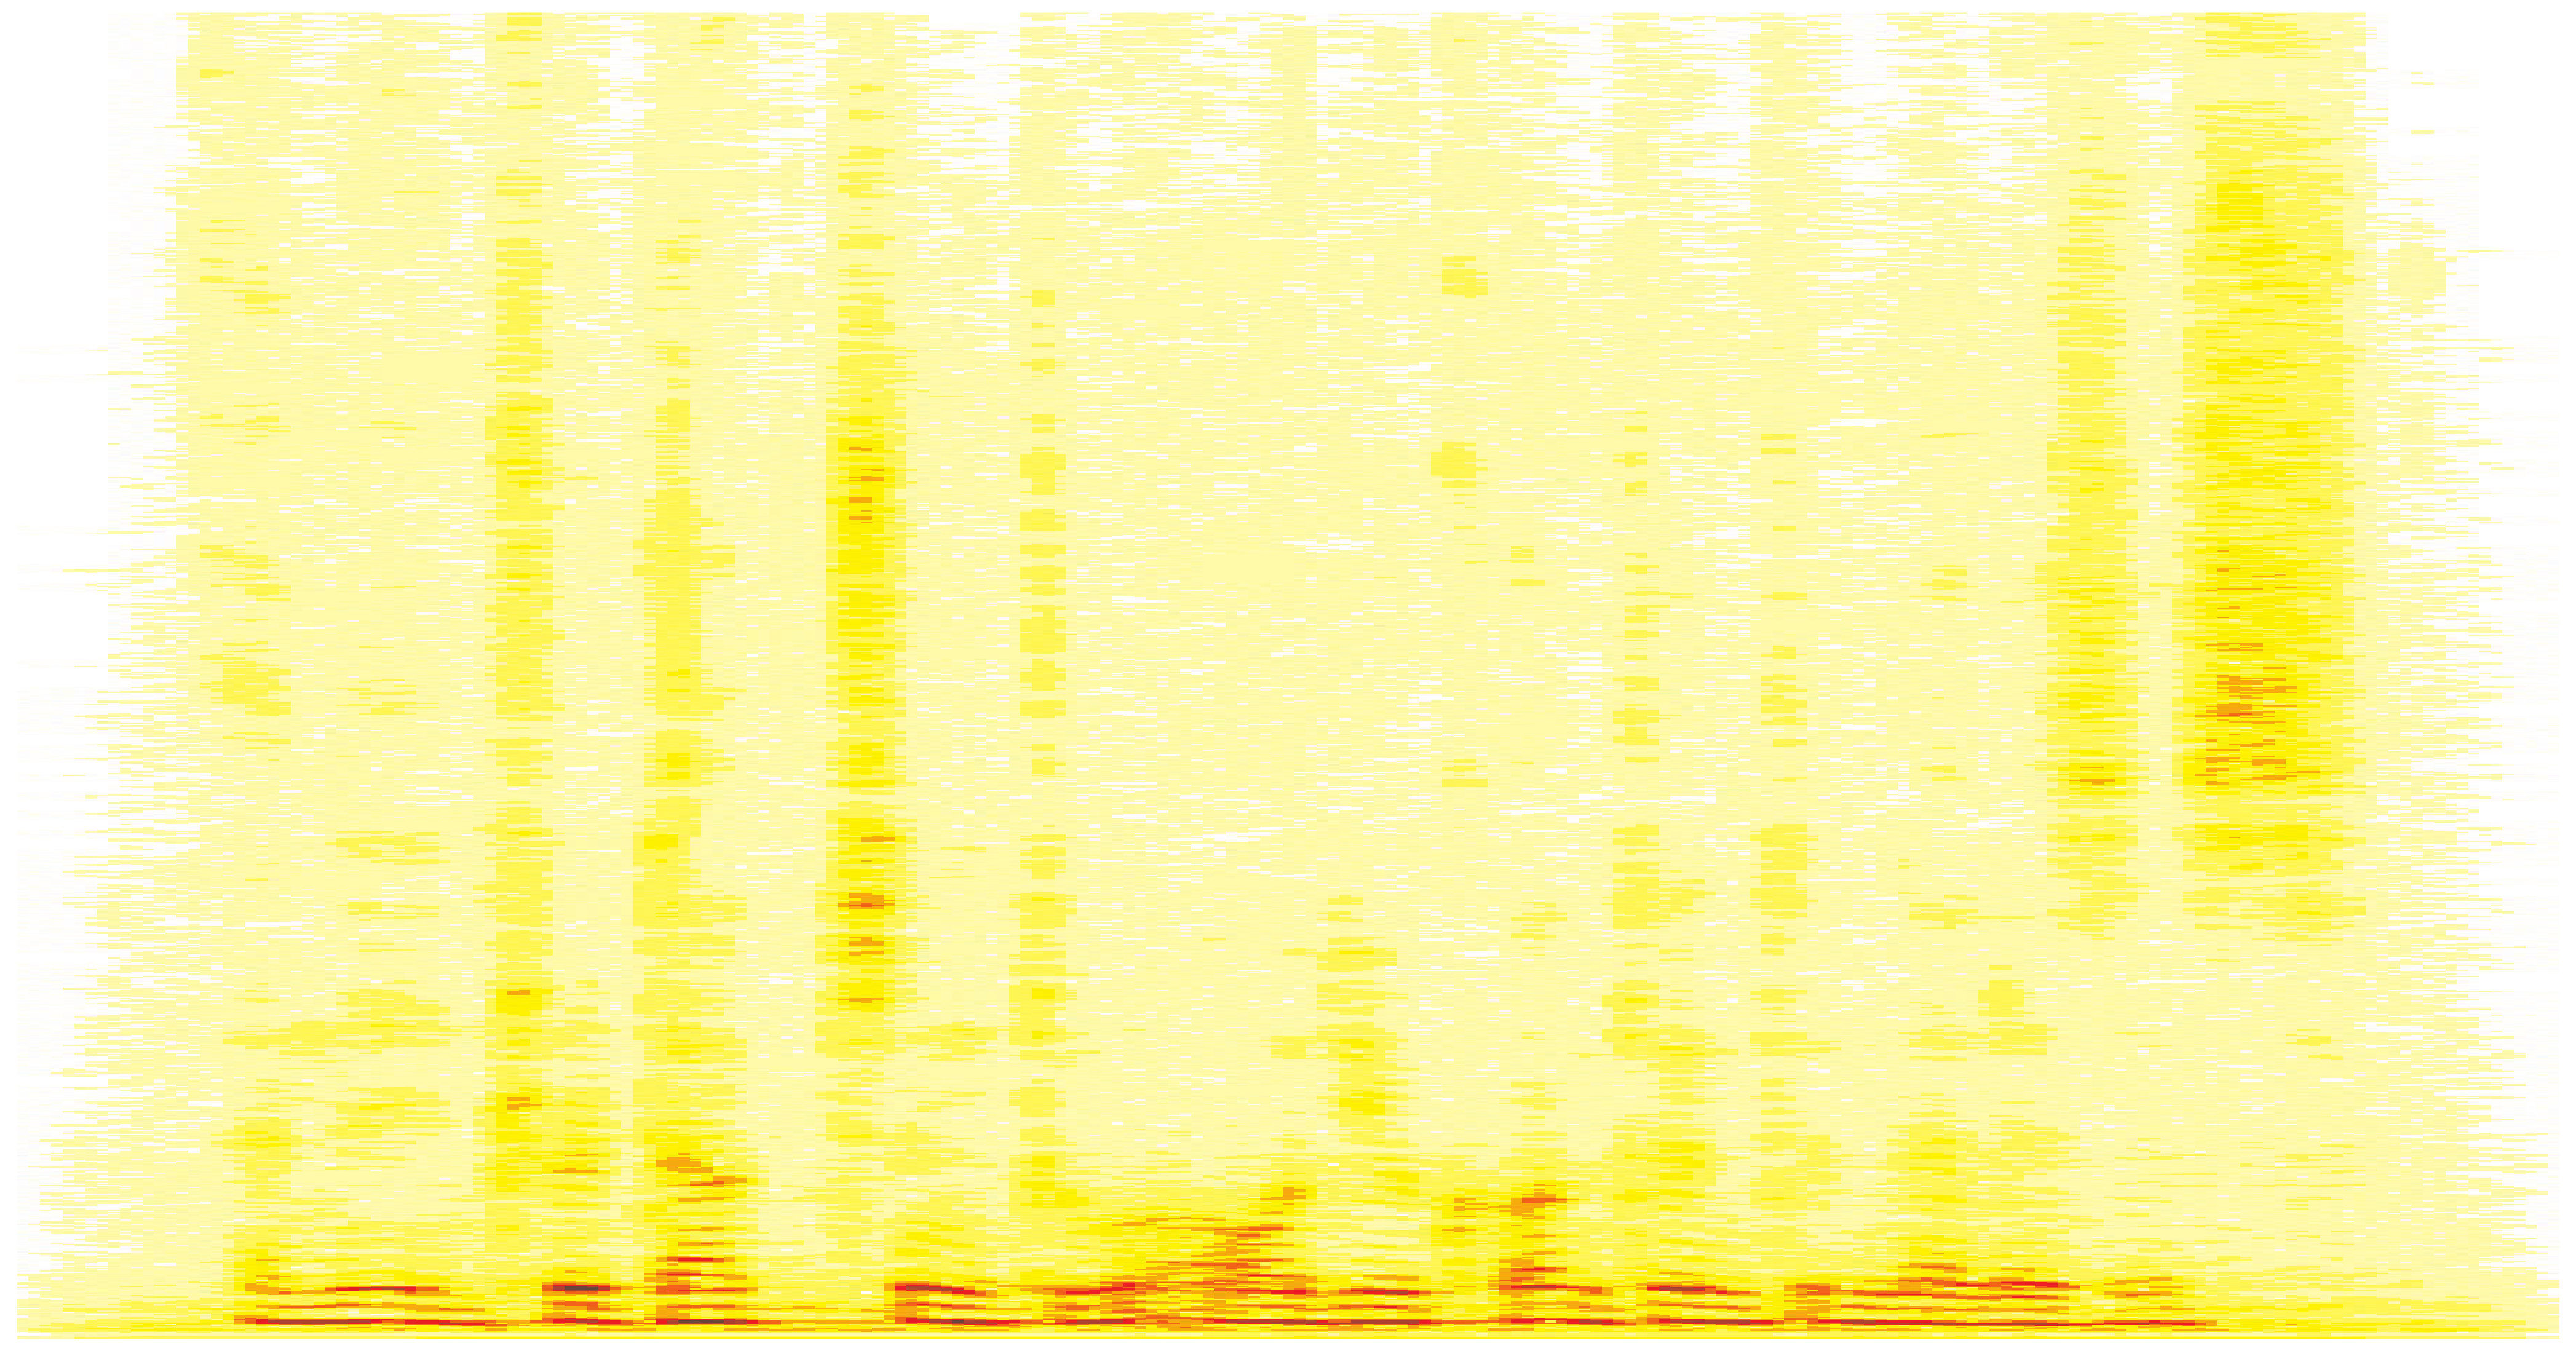
\includegraphics[width=\textwidth,height=3cm]{title}}

%%%%%%%%%%%%%%%%%%%%%%%%%%%%%%%%%%%%%%%%%%%%%%%%%%%%%%%%%%%%%%%%%%%%%%%%%%%%%%%%%%
%%%%%%%%%%%%%%%%%%%%%%%%%%%%%%%%%%%%%%%%%%%%%%%%%%%%%%%%%%%%%%%%%%%%%%%%%%%%%%%%%%
% colors
\definecolor{gtgold}{HTML}{E0AA0F} %{rgb}{0.88,0.66,1,0.06} [234, 170, 0]/256

%%%%%%%%%%%%%%%%%%%%%%%%%%%%%%%%%%%%%%%%%%%%%%%%%%%%%%%%%%%%%%%%%%%%%%%%%%%%%%%%%%
%%%%%%%%%%%%%%%%%%%%%%%%%%%%%%%%%%%%%%%%%%%%%%%%%%%%%%%%%%%%%%%%%%%%%%%%%%%%%%%%%%
% math
\DeclareMathOperator*{\argmax}{argmax}
\DeclareMathOperator*{\argmin}{argmin}
\DeclareMathOperator*{\atan}{atan}
\DeclareMathOperator*{\arcsinh}{arcsinh}
\DeclareMathOperator*{\sign}{sign}
\DeclareMathOperator*{\tcdf}{tcdf}
\DeclareMathOperator*{\si}{sinc}
\DeclareMathOperator*{\princarg}{princarg}
\DeclareMathOperator*{\arccosh}{arccosh}
\DeclareMathOperator*{\hwr}{HWR}
\DeclareMathOperator*{\flip}{flip}
\DeclareMathOperator*{\sinc}{sinc}
\DeclareMathOperator*{\floor}{floor}
\newcommand{\e}{{e}}
\newcommand{\jom}{\mathrm{j}\omega}
\newcommand{\jOm}{\mathrm{j}\Omega}
\newcommand   {\mat}[1]    		{\boldsymbol{\uppercase{#1}}}		%bold
\renewcommand {\vec}[1]    		{\boldsymbol{\lowercase{#1}}}		%bold

%%%%%%%%%%%%%%%%%%%%%%%%%%%%%%%%%%%%%%%%%%%%%%%%%%%%%%%%%%%%%%%%%%%%%%%%%%%%%%%%%%
%%%%%%%%%%%%%%%%%%%%%%%%%%%%%%%%%%%%%%%%%%%%%%%%%%%%%%%%%%%%%%%%%%%%%%%%%%%%%%%%%%
% media9
\newcommand{\includeaudio}[1]{{\includemedia[
                        addresource=audio/#1.mp3,
                        width=5mm,
                        height=5mm,
                        activate=onclick,
                        flashvars={
                            source=audio/#1.mp3  
                            &autoPlay=true
                        }]
                        {
\includegraphics[width=5mm, height=5mm]{SpeakerIcon}}
                        {APlayer.swf}}}
\newcommand{\audioautoplay}[1]{{\begin{center}\includemedia[
                            addresource=audio/#1.mp3,
                            width=.1\linewidth,
                            height=.01\linewidth,
                            activate=pageopen,
                            flashvars={
                                source=audio/#1.mp3  
                                &autoPlay=true
                            }]
                            {}
                            {APlayer.swf}\end{center}}}

\newcommand{\includevideo}[1]{{\begin{center}\includemedia[
                        addresource=video/#1.mp4,
                        width=0.8\linewidth,
                        height=0.4\linewidth,
                        activate=onclick,
                        flashvars={
                            source=video/#1.mp4  
                            &autoPlay=true
                        }]
                        {}
                        {VPlayer.swf}\end{center}}}
\newcommand{\videowithmatlab}[1]{{\begin{center}\includemedia[
                        addresource=video/animate#1.mp4,
                        width=0.8\linewidth,
                        height=0.4\linewidth,
                        activate=onclick,
                        flashvars={
                            source=video/animate#1.mp4  
                            &autoPlay=true
                        }]
                        {}
                        {VPlayer.swf}\end{center}\addreference{matlab source: matlab/animate#1.m}}}
                        

%%%%%%%%%%%%%%%%%%%%%%%%%%%%%%%%%%%%%%%%%%%%%%%%%%%%%%%%%%%%%%%%%%%%%%%%%%%%%%%%%%
%%%%%%%%%%%%%%%%%%%%%%%%%%%%%%%%%%%%%%%%%%%%%%%%%%%%%%%%%%%%%%%%%%%%%%%%%%%%%%%%%%
% other commands
\newcommand{\question}[1]{%\vspace{-4mm}
                          \setbeamercovered{invisible}
                          \begin{columns}[T]
                            \column{.8\textwidth}
                                \textbf{#1}
                            \column{.2\textwidth}
                                \vspace{-8mm}
                                \begin{flushright}
                                     
\includegraphics[scale=.5]{question_mark}
                                \end{flushright}
                                \vspace{6mm}
                          \end{columns}\pause\vspace{-12mm}}

\newcommand{\toremember}[1]{%\vspace{-4mm}
                          \begin{columns}[T]
                            \column{.8\textwidth}
                                \textbf{#1}
                            \column{.2\textwidth}
                                \vspace{-4mm}
                                \begin{flushright}
                                     
\includegraphics[scale=.5]{exclamation_mark}
                                \end{flushright}
                                \vspace{6mm}
                          \end{columns}\vspace{-6mm}}

\newcommand{\matlabexercise}[1]{%\vspace{-4mm}
                          \setbeamercovered{invisible}
                          \begin{columns}[T]
                            \column{.8\textwidth}
                                \textbf{matlab exercise}: #1
                            \column{.2\textwidth}
                                \begin{flushright}
                                     
\includegraphics[scale=.5]{logo_matlab}
                                \end{flushright}
                                %\vspace{6mm}
                          \end{columns}}

\newcommand{\addreference}[1]{  
                  
                    \begin{textblock*}{\baselineskip }(1.12\textwidth,.3\textheight) %(1.15\textwidth,.4\textheight)
                        \rotatebox{90}{\tiny {#1}}
                    \end{textblock*}}
                    
\newcommand{\figwithmatlab}[1]{
                    \begin{figure}
                        \centering
                        \includegraphics{#1}
                        %\label{fig:#1}
                    \end{figure}
                    
                    \addreference{matlab source: \href{https://github.com/alexanderlerch/ACA-Slides/blob/master/matlab/display#1.m}{matlab/display#1.m}}}
\newcommand{\figwithref}[2]{
                    \begin{figure}
                        \centering
                        \includegraphics{#1}
                        \label{fig:#1}
                    \end{figure}
                    
                    \addreference{#2}}  
                                    
\newcommand{\inserticon}[1]{

                    \begin{textblock*}{100mm}(14.5cm,7.5cm)
                        \includegraphics[height=.8cm,keepaspectratio]{#1}
                    \end{textblock*}}            

%%%%%%%%%%%%%%%%%%%%%%%%%%%%%%%%%%%%%%%%%%%%%%%%%%%%%%%%%%%%%%%%%%%%%%%%%%%%%%%%%%
%%%%%%%%%%%%%%%%%%%%%%%%%%%%%%%%%%%%%%%%%%%%%%%%%%%%%%%%%%%%%%%%%%%%%%%%%%%%%%%%%%
% counters
\newcounter{i}
\newcounter{j}
\newcounter{iXOffset}
\newcounter{iYOffset}
\newcounter{iXBlockSize}
\newcounter{iYBlockSize}
\newcounter{iYBlockSizeDiv2}
\newcounter{iDistance}



\subtitle{Module 8.0: Classifiers}

%%%%%%%%%%%%%%%%%%%%%%%%%%%%%%%%%%%%%%%%%%%%%%%%%%%%%%%%%%%%%%%%%%%%%%%%%%%%
\begin{document}
    % generate title page
	

\begin{frame}
    \titlepage
    %\vspace{-5mm}
    \begin{flushright}
        \href{http://www.gtcmt.gatech.edu}{\includegraphics[height=.8cm,keepaspectratio]{logo_GTCMT_black}}
    \end{flushright}
\end{frame}


    \section[overview]{lecture overview}
        \begin{frame}{introduction}{overview}
            \begin{block}{corresponding textbook section}
                    \href{http://ieeexplore.ieee.org/xpl/articleDetails.jsp?arnumber=6331125}{Chapter 8: Musical Genre, Similarity, and Mood} (pp.~155)
            \end{block}

            \begin{itemize}
                \item   \textbf{lecture content}
                    \begin{itemize}
                        \item   training set and test set
                        \item   intuitive intro to machine learning
                        \item   classifier examples
                    \end{itemize}
                \bigskip
                \item<2->   \textbf{learning objectives}
                    \begin{itemize}
                        \item   describe the basic principles and challenges of data-driven machine learning approaches
                        \item   implement a kNN classifier in Matlab
                    \end{itemize}
            \end{itemize}
            \inserticon{directions}
        \end{frame}

    \section[intro]{introduction}
        \begin{frame}{classification}{machine learning}
            \begin{itemize}
                \item   computer runs a 'generic' program
                \item   adapts parameters to training data
                \bigskip
                \item[$\Rightarrow$] \textbf{data driven} approach
                
                \bigskip
                \item<2->[] data and its representation defines much of the outcome
                    \begin{itemize}
                        \item   \textit{validity}: is data representative sample and do features focus on important characteristics
                        \item   \textit{reliability}: does data lead to accurate and consistent results
                        \item   \textit{reproducibility}: will multiple runs result in similar results
                    \end{itemize}
            \end{itemize}
        \end{frame}
        \begin{frame}{classification}{general steps}
            \begin{enumerate}
                \item	\textbf{define training set}: annotated results
                \smallskip
                \item<2->	\textbf{normalize} training set
                \smallskip
                \item<3->	\textbf{train} classifier
                \smallskip
                \item<4->	\textbf{evaluate} classifier with test (or validation) set
                \smallskip
                \item<5->	(\textbf{adjust} classifier settings, return to 4.)
            \end{enumerate}
        \end{frame}
        
    \section{classification}
        \begin{frame}{classification}{rules of thumb}
            \vspace{-3mm}
            \begin{itemize}
                \item   \textbf{training set}
                    \begin{itemize}
                        \item	training set size vs.\ number of features
                            \begin{itemize}
                                \item	training set too small,% $\Rightarrow$ \textit{overfitting}
                                feature number too large $\Rightarrow$ \textit{overfitting}
                            \end{itemize}
                        \item<1->	training set \textbf{too noisy} $\Rightarrow$ \textit{underfitting}
                        \item<1->	training set \textbf{not representative} $\Rightarrow$ \textit{bad classification performance}
                    \end{itemize}
                \smallskip
                \item<2->   \textbf{classifier}
                    \begin{itemize}
                        \item<2->   classifier too complex $\Rightarrow$ \textit{overfitting}
                        \item<2->	\textbf{poor classifier} $\Rightarrow$ \textit{bad classification performance}
                            \begin{itemize}
                                \item[$\rightarrow$]	different classifier
                            \end{itemize}
                    \end{itemize}
                \smallskip
                \item<3->   \textbf{features}
                    \begin{itemize}
                        \item<3->	\textbf{poor features} $\Rightarrow$ \textit{bad classification performance}
                            \begin{itemize}
                                \item[$\rightarrow$]	new, better features
                            \end{itemize}
                        \item<3->	features \textbf{not normalized} $\Rightarrow$ possibly \textit{bad classification performance}
                            \begin{itemize}
                                \item	feature distribution (range, mean, symmetry)
                            \end{itemize}
                    \end{itemize}
            \end{itemize}
        \end{frame}
        \begin{frame}{musical genre classification}{classifier: evaluation}
            \begin{itemize}
                \item	define \textbf{test set} for evaluation
                    \begin{itemize}
                        \item	test set \textit{different} from training set
                        \item	otherwise, same requirements
                    \end{itemize}
                
                \bigskip
                \item<2->	example: \textbf{$N$-fold cross validation}
                    \begin{enumerate}
                        \item<2->	split training set into $N$ parts (randomly, but preferably identical number per class)
                        \item<3->	select one part as test set
                        \item<4->	train the classifier with all observations from remaining $N-1$ parts
                        \item<5->	compute the classification rate for the test set
                        \item<6->	repeat until all $N$ parts have been tested
                        \item<7->	overall result: \textit{average} classification rate
                    \end{enumerate}
            \end{itemize}
        \end{frame}
        
     \section{classifier examples}
        \begin{frame}{musical genre classification}{classifier: kNN}
            \begin{columns}
                \column{.6\linewidth} 
                    \begin{itemize}
                        \item	\textbf{training}: extract reference vectors from training set (keep class labels)
                        \item<2->	\textbf{classification}: extract test vector and set class to majority of $k$ nearest reference vectors
                        \bigskip
                        \item<6->	\textbf{classifier data}: all training vectors
                    \end{itemize}
                \column{.4\linewidth} 
                    \only<1,6>{\begin{figure}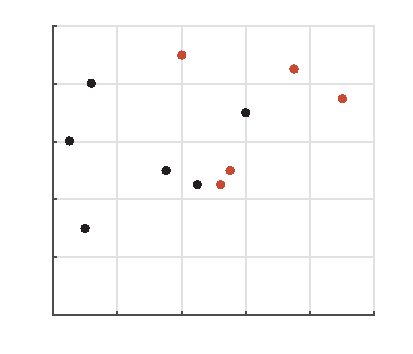
\includegraphics[width=\columnwidth]{Knn-0}\end{figure}}
                    \setcounter{i}{1}
                    \setcounter{j}{2}
                    \whiledo{\value{i}<5}
                    {
                        \only<\value{j}>{\begin{figure}\includegraphics[width=\columnwidth]{Knn-\arabic{i}}\end{figure}}
                        \stepcounter{i}
                        \stepcounter{j}
                    }
                    \only<3>{$k = 3 \Rightarrow$ red majority}
                    \only<4>{$k = 5 \Rightarrow$ black majority}
                    \only<5>{$k = 7 \Rightarrow$ red majority}
            \end{columns}
            \addreference{matlab source: \href{https://github.com/alexanderlerch/ACA-Slides/blob/master/matlab/displayKnn.m}{matlab/displayKnn.m}}
        \end{frame}
        \begin{frame}{musical genre classification}{classifier: GMM}
            \vspace{-3mm}
            \begin{itemize}
                \item	\textbf{training}: build model of each class distribution as superposition of Gaussian distributions
                \item<2->	\textbf{classification}: compute output of each Gaussian and select class with highest probability
                    \only<2>{
                        \vspace{-1mm}
                        \figwithmatlab{Gmm}
                        }
                \item<3->	\textbf{classifier data}: per class per Gaussian: $\mu$ and covariance, mixture weight?
            \end{itemize}
        \end{frame}
        \begin{frame}{musical genre classification}{classifier: SVM}
            \begin{itemize}
                \item	\textbf{training}:
                    \begin{itemize}
                        \item   map features to high dimensional space
                            \figwithref{SVM}{\href{https://en.wikipedia.org/wiki/Support\_vector\_machine}{https://en.wikipedia.org/wiki/Support\_vector\_machine}}
                        \item   find separating hyperplane through maximum distance of support vectors (data points)
                    \end{itemize}
                \item<2->	\textbf{classification}: apply feature transform and proceed with 'linear' classification
                \item<3->	\textbf{classifier data}: support vectors, kernel, kernel parameters
            \end{itemize}
        \end{frame}
    
    \section{summary}
        \begin{frame}{summary}{lecture content}
            \begin{itemize}
                \item   \textbf{data-driven approach}
                    \begin{itemize}
                        \item   general systems that learn behavior from data
                        \item   human interaction through
                            \begin{itemize}
                                \item   parametrization and procedures
                                \item   data selection
                            \end{itemize}
                    \end{itemize}
                \bigskip
                \item   \textbf{training \& test set}
                    \begin{enumerate}
                        \item   must not overlap
                        \item   must be representative
                    \end{enumerate}
                \bigskip
                \item   \textbf{fine balance of inputs}
                    \begin{enumerate}
                        \item   number of features
                        \item   classifier complexity
                        \item   amount and variability of data
                    \end{enumerate}
            \end{itemize}
            \inserticon{summary}
        \end{frame}
\end{document}
